% !TEX program = pdflatex
%%%%%%%%%%%%%%%%%%%%%%%%%%%%%%%%%%%%%%%%%
% Structured General Purpose Assignment
% LaTeX Template
%
% This template has been downloaded from:
% http://www.latextemplates.com
%
% Original author:
% Ted Pavlic (http://www.tedpavlic.com)
%
% Note:
% The \lipsum[#] commands throughout this template generate dummy text
% to fill the template out. These commands should all be removed when
% writing assignment content.
%
%%%%%%%%%%%%%%%%%%%%%%%%%%%%%%%%%%%%%%%%%

%----------------------------------------------------------------------------------------
%	PACKAGES AND OTHER DOCUMENT CONFIGURATIONS
%----------------------------------------------------------------------------------------

\documentclass{article}

\usepackage{fancyhdr} % Required for custom headers
\usepackage{lastpage} % Required to determine the last page for the footer
\usepackage{extramarks} % Required for headers and footers
\usepackage{graphicx} % Required to insert images
\usepackage{subcaption}
\usepackage{lipsum} % Used for inserting dummy 'Lorem ipsum' text into the template

\usepackage[utf8]{inputenc}
\usepackage[ngerman,english]{babel}
\usepackage[T1]{fontenc}
\usepackage{breakurl}
\usepackage[hyphens]{url}
\usepackage{color}
\usepackage{float}
\usepackage{hyperref}
\usepackage{tabularx}
\usepackage{enumitem}
\usepackage{color, colortbl}
\usepackage[super]{nth}

\usepackage[
	backend=biber,
	style=numeric-comp,
	natbib=true,
	url=false,
	doi=false,
	eprint=false,
	sorting=none,
	isbn=false]
	{biblatex}

\bibliography{references}

\addto\captionsenglish{
  \renewcommand{\contentsname}%
    {Table of Contents}%
}

% Margins
\topmargin=-0.45in
\evensidemargin=0in
\oddsidemargin=0in
\textwidth=6.5in
\textheight=9.0in
\headsep=0.25in

\linespread{1.1} % Line spacing
% Set up the header and footer
\pagestyle{fancy}
\lhead{} % Top left header
\chead{Pattern in Software Engineering Summary} % Top center header
\rhead{\firstxmark} % Top right header
\lfoot{\lastxmark} % Bottom left footer
\cfoot{} % Bottom center footer
\rfoot{Page\ \thepage\ of\ \pageref{LastPage}} % Bottom right footer
\renewcommand\headrulewidth{0.4pt} % Size of the header rule
\renewcommand\footrulewidth{0.4pt} % Size of the footer rule

\setlength\parindent{0pt} % Removes all indentation from paragraphs

\hypersetup{	% Remove red boxes around links in table of contents
	pdfborder={0 0 0}
}


\begin{document}
\setcounter{tocdepth}{3}

%----------------------------------------------------------------------------------------
% TITLE PAGE
%----------------------------------------------------------------------------------------
\pagenumbering{gobble}
% \maketitle
\begin{titlepage}
  \centering
\includegraphics[width=5cm]{tumlogo}

  \vspace{2.5cm}
  \Huge{Pattern in Software Engineering} \\
  \vspace{0.1in}\huge{Lecture Summary}\\

  \Large
  \vspace{1.5cm}
  \begin{tabularx}{9cm}{r l}
    Authors: & Thomas Pettinger \\
    & Nils Kunze\\
    & Benedikt Schlagberger\\
  \end{tabularx}

  \vfill
  \textbf{2016-02-22} \\
  \vspace{0.3in}\normalsize{Pattern in Software Engineering}\\
  \vspace{0.03in}\normalsize{\textsc{Technische Universität München}}\\
  \vspace{1cm}

\end{titlepage}
%----------------------------------------------------------------------------------------


\newpage
\thispagestyle{empty}
\tableofcontents

\newpage
\pagenumbering{arabic}

%!TEX root = ../report.tex

\section{Design Patterns}


\subsection{Structural Patterns}

\subsubsection{Adapter Pattern/Wrapper}
Connects incompatible components to for example
\begin{itemize}
  \item Reuse existing components
  \item Convert an interface to another interface (maybe needed by an API call)
\end{itemize}

Structure:\\
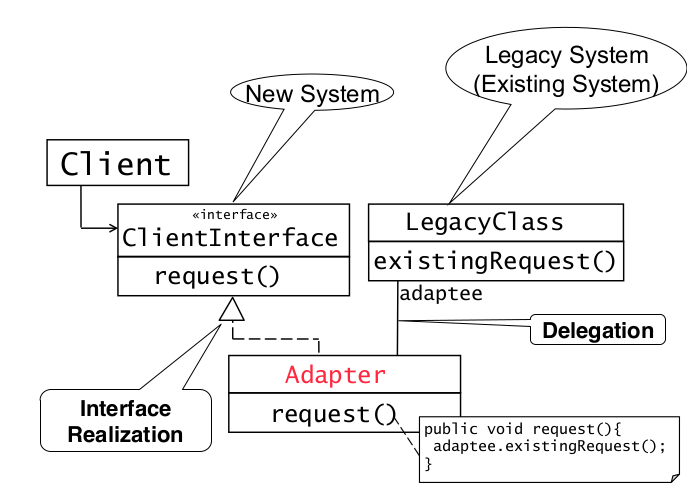
\includegraphics[width=\linewidth]{images/pattern_adapter.png}
\newpage

\subsubsection{Bridge Pattern}
Allows to delay the assignment of an implementation of an interface from compile to run time.\\
Structure:\\
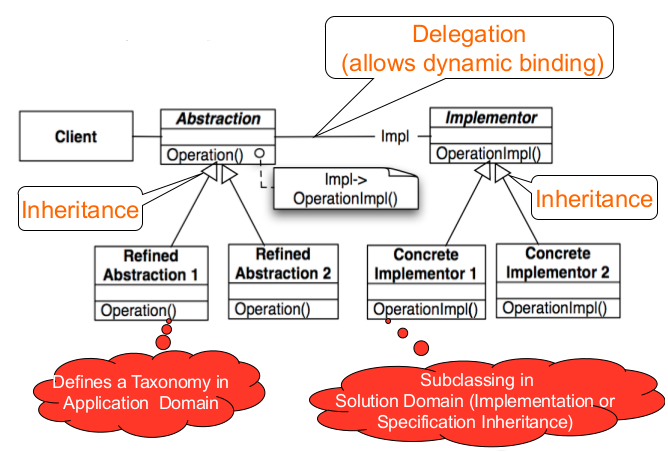
\includegraphics[width=\linewidth]{images/pattern_bridge.png}
The \textbf{degenerated bridge pattern} is the same as the bridge pattern without the taxonomy in the application domain.
\newpage

\subsubsection{Proxy Pattern/Caching}
The proxy pattern allows to defer object creation and object initialization to the time you need the object (Remote Proxy (Caching), Substitute (Virtual Proxy), Protection Proxy (Access control/Firewall)).\\
Structure:\\
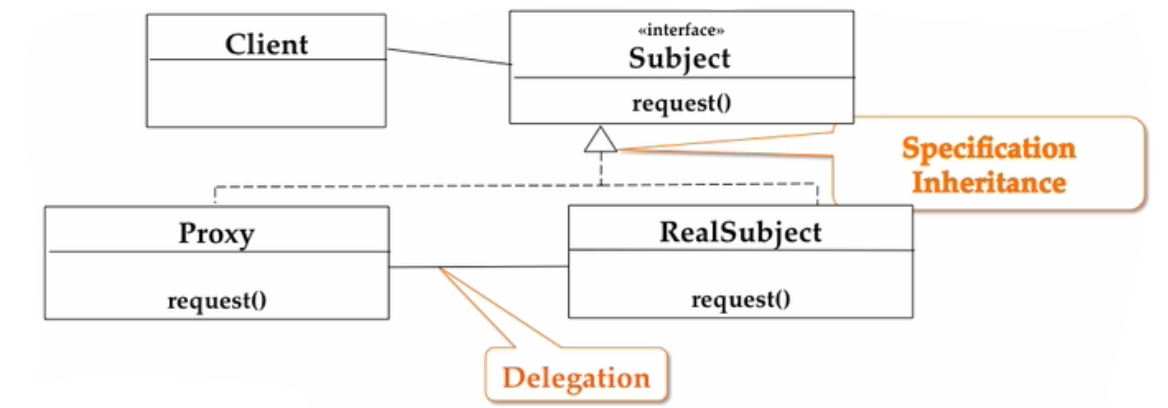
\includegraphics[width=\linewidth]{images/pattern_proxy.png}
The client never calls request() in RealSubject, instead it always calls the method in Proxy which might delegate it to the RealSubject.
\newpage

\subsubsection{Composite Pattern}
The composite pattern models tree structures that represent part-whole hierarchies with arbitrary depth and width.
It lets the client treat individual objects and groups uniformly. \\
Structure:\\
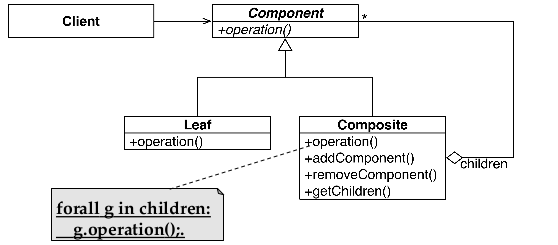
\includegraphics[width=\linewidth]{images/pattern_composite.png}
\newpage


\subsection{Behavioral Patterns}

\subsubsection{Strategy Pattern}
Suited for situations where different algorithms are available for a problem (e.g. sorting).\\
Structure:\\
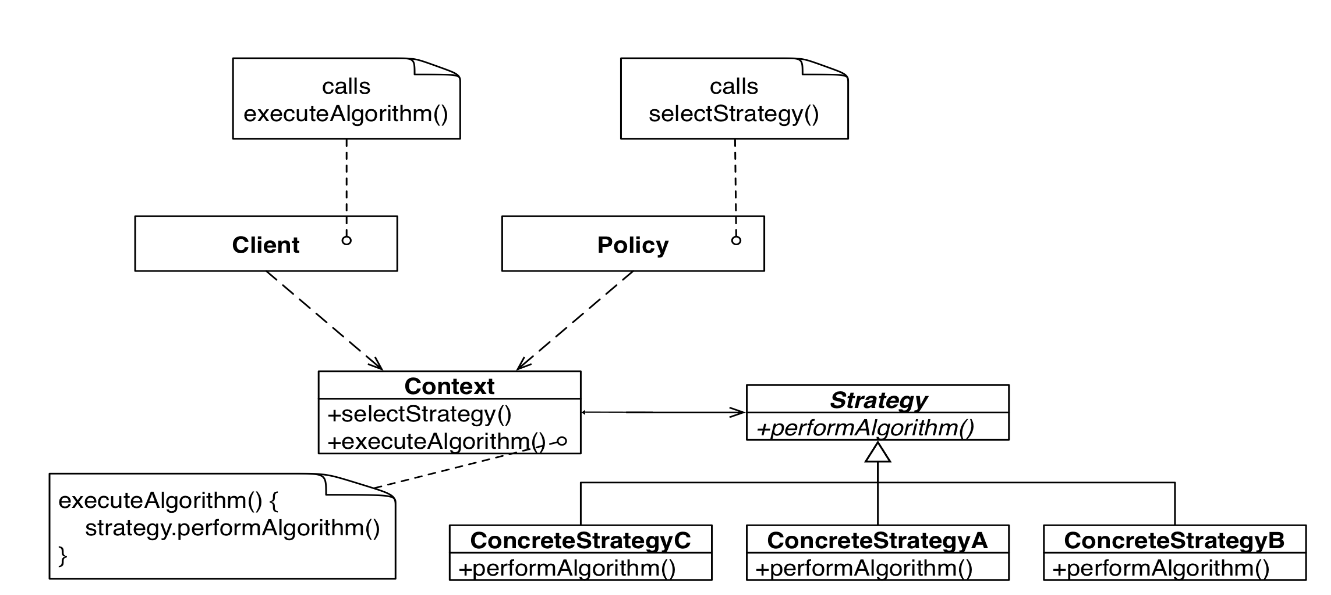
\includegraphics[width=\linewidth]{images/pattern_strategy.png}
A strategy is chosen on \textbf{runtime} by the Policy class before the client calls executeAlgorithm.
\newpage

\subsubsection{State Pattern}
Dependent on the current state of a system, an action should do different things (e.g. TCP open, close).
The state pattern avoids many if else statements and is flexible to add more cases/states.\\
Structure:\\
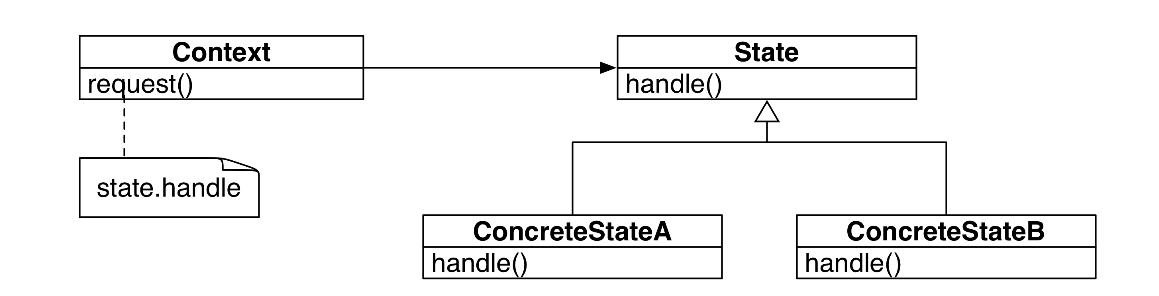
\includegraphics[width=\linewidth]{images/pattern_state.png}
Problem: Where are state transactions handled? (in the exercise of the lecture in the states)
\newpage

\subsubsection{Observer Pattern}
The observer pattern handles changes in a publisher class and notifies all subscribers about that change (e.g. the user interface) to maintain consistency.
There are three variants for maintaining consistency:
\begin{itemize}
  \item \textbf{Push Notification:} Every time a state changes, all subscribers are notified
  \item \textbf{Push-Update Notification:} The publisher also sends the state that has changed
  \item \textbf{Pull Notification:} A subscriber inquires about the state of the publisher
\end{itemize}
Structure:\\
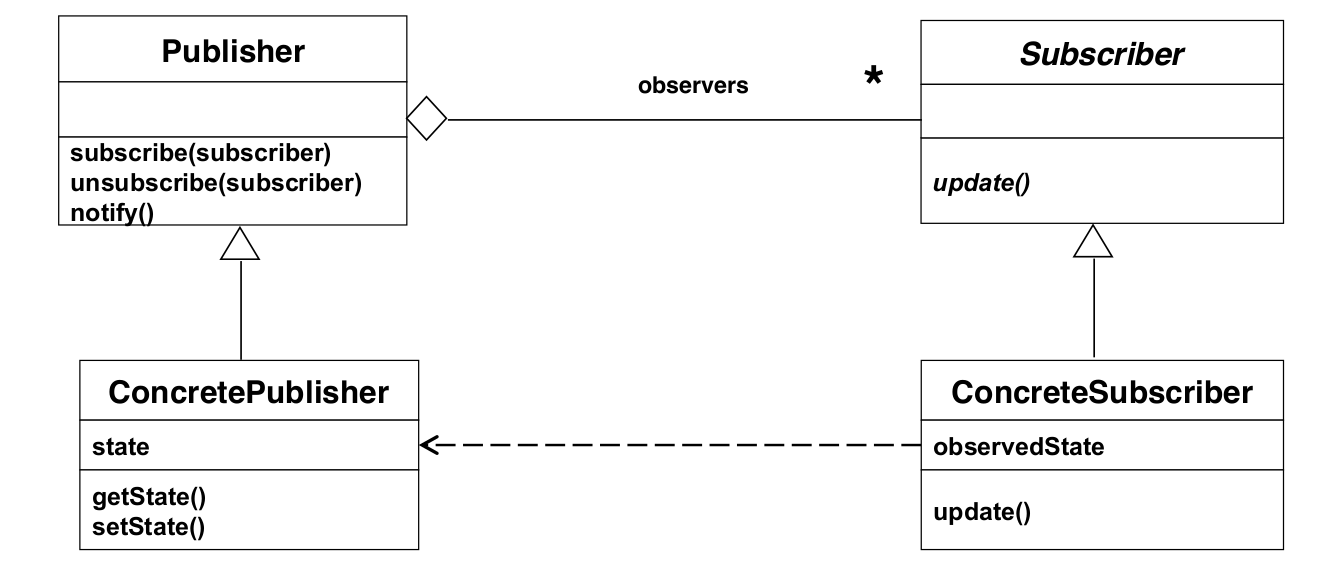
\includegraphics[width=\linewidth]{images/pattern_observer.png}
\newpage

\subsubsection{Model View Controller Pattern}
The model-view-controller architectural style decouples data access and data representation.
The view handles the data representation, the model the data access and the controller handles the communication between the other two.\\
Structure:\\
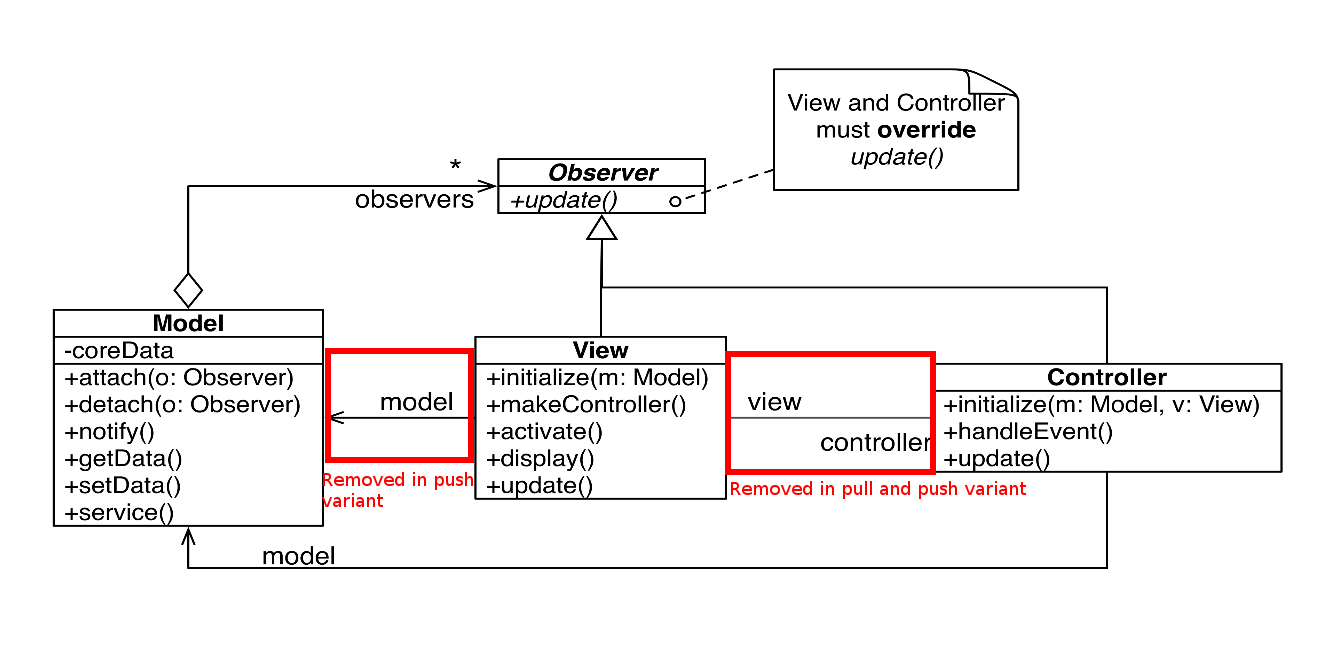
\includegraphics[width=\linewidth]{images/pattern_mvc.png}
In the \textbf{pull variant} the connection between the controller and the view is removed.
In this variant the view asks the model for the data explicitly.\\
In the \textbf{push notification variant} both the connection between the view and the model and controller respectively are removed.
When a change in the model occurs, the view and the controller are updated via the observer pattern.
\newpage

\subsubsection{Command Pattern}
The command pattern is used for designing user interfaces with multiple commands without using multiple if statements (if(command == x) {...} else if(command == y) ...).
It can be used to make menus reusable across applications.\\
Structure:\\
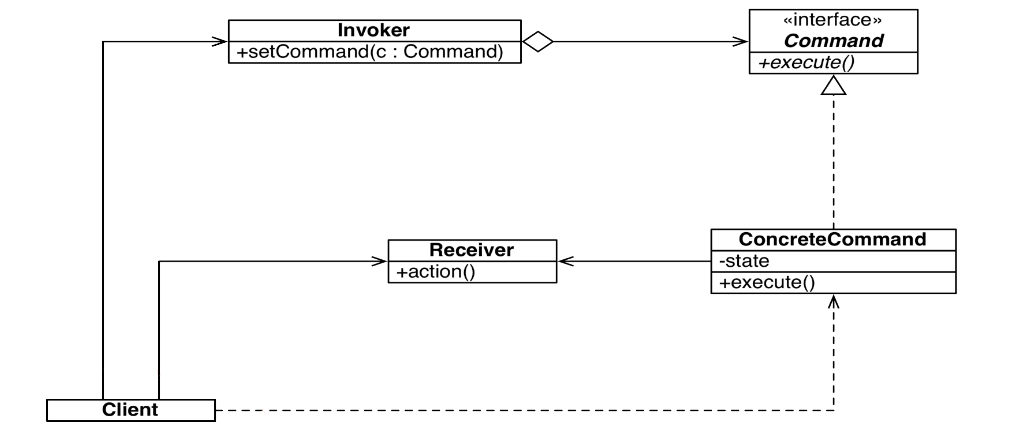
\includegraphics[width=\linewidth]{images/pattern_command.png}
Commands as classes allow command histories and thus undo and redo.\\
Common Applications:
\begin{itemize}
  \item \textbf{Command Manager} Central repository for all commands
  \item \textbf{Redo/Undo Manager}
  \item \textbf{Queue} Holds commands until others objects are ready to do something with them
  \item \textbf{Dispatcher} (e.g. keyboard event loop)
\end{itemize}
\newpage


\subsection{Creational Patterns}

\subsubsection{Factory Pattern}
A factory class handles the instantiation of objects inheriting from one superclass depending on a keyword or value.\\
Structure:\\
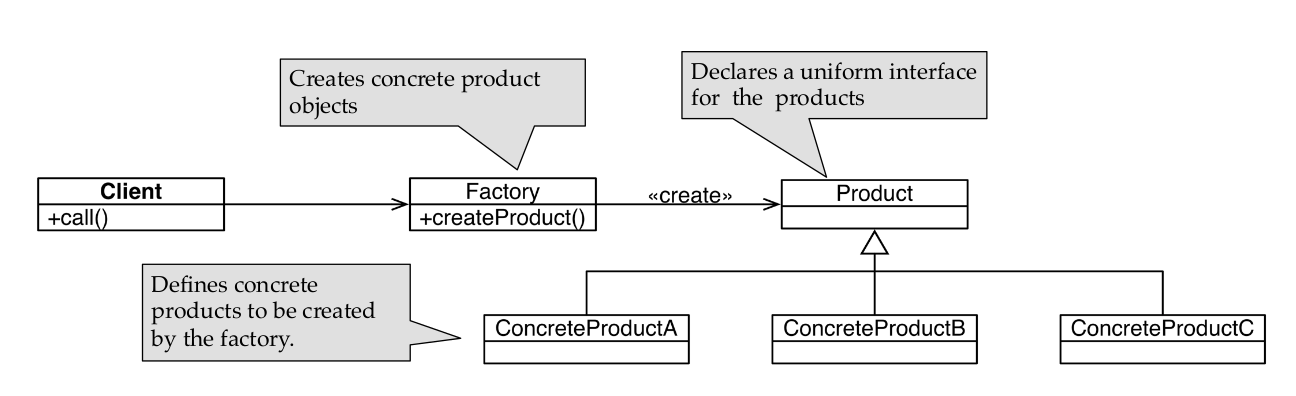
\includegraphics[width=\linewidth]{images/pattern_factory.png}
\newpage

\subsubsection{Abstract Factory Pattern}
The abstract factory pattern is used to instantiate or initialize an object consisting of more subparts.
Every implementation of the abstract factory creates a set of components consisting of a variant of every part of the whole object.
Structure:\\
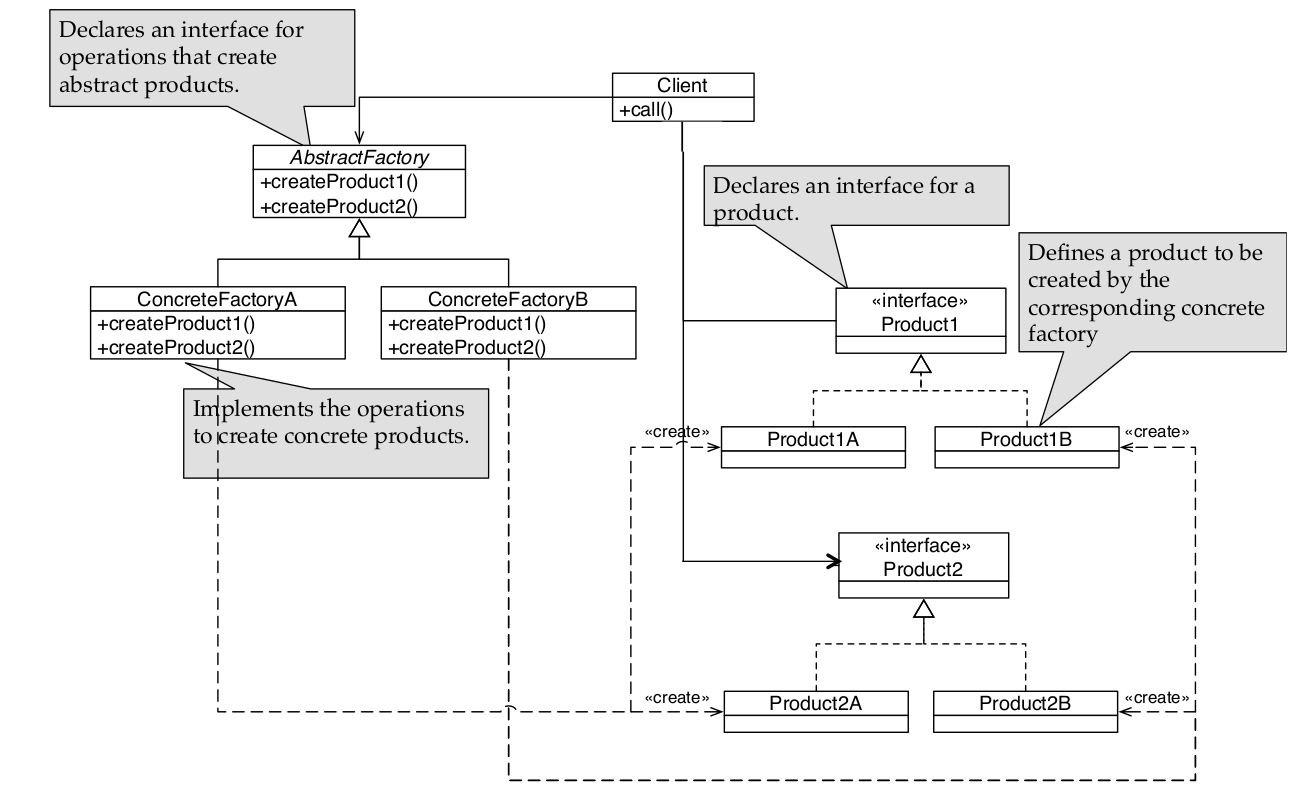
\includegraphics[width=\linewidth]{images/pattern_abstract_factory.png}
\newpage

%!TEX root = ../report.tex

\section{Architectural Patterns}

\subsection{Layer Pattern}
Structure:\\
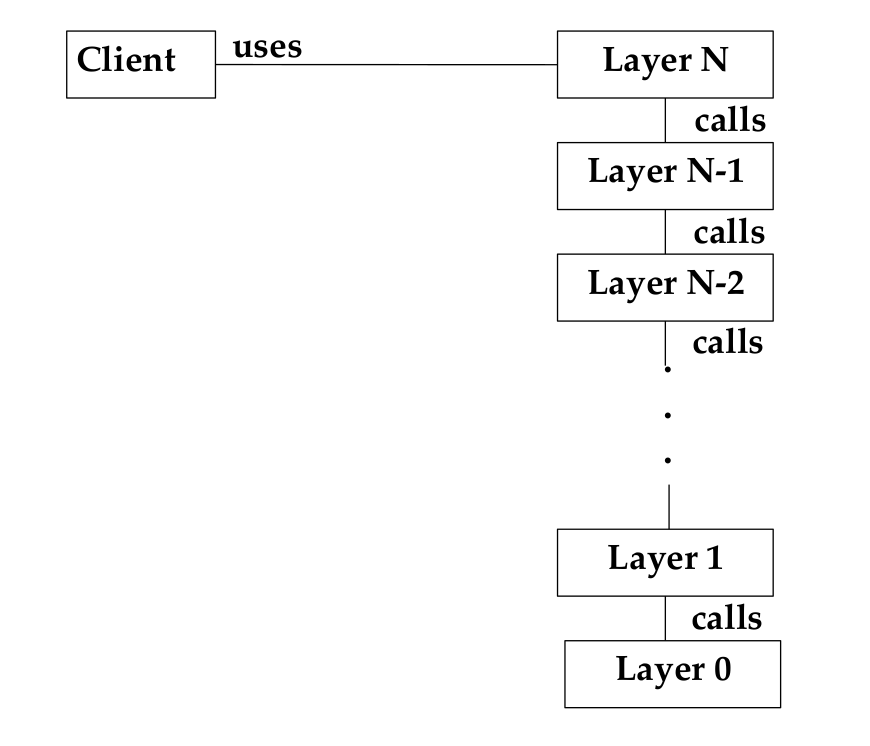
\includegraphics[width=.75\linewidth]{images/pattern_layer.png}
\begin{description}
  \item[Closed Architecture (Opaque Layering):]\hfill \\
    Each layer can only call operations from the layer below.\\
  \item[Open Architecture (Transparent Layering):]\hfill \\
    Each layer can call operations from \textbf{any} layer below
\end{description}

\textbf{5 Steps to Create a Layered Architecture}
\begin{enumerate}
  \item Identify subsystems
  \item Structure the individual layers
  \item Specify the communication protocol between adjacent layers (push/pull)
  \item Decouple adjacent layers
  \item Design an error-handling strategy (try handling errors on lowest possible layer)
\end{enumerate}
\newpage

\subsection{Repository Pattern}
The repository pattern is used to support a collection of independent programs that work cooperatively on a common data structure called the repository.
The control flow is not specified by the pattern.\\
Structure:\\
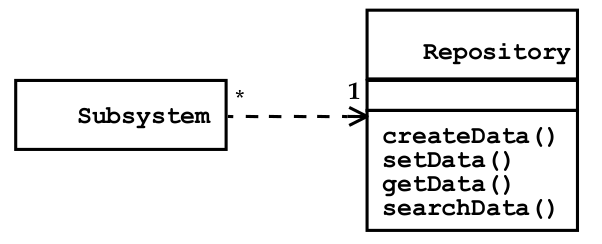
\includegraphics[width=.75\linewidth]{images/pattern_repository.png}
\newpage

\subsection{Blackboard Pattern}
Experts throwing knowledge onto a blackboard (repository) which might be correct or not. Some can be extracted to higher order knowledge and other might be rejected.\\
Structure:\\
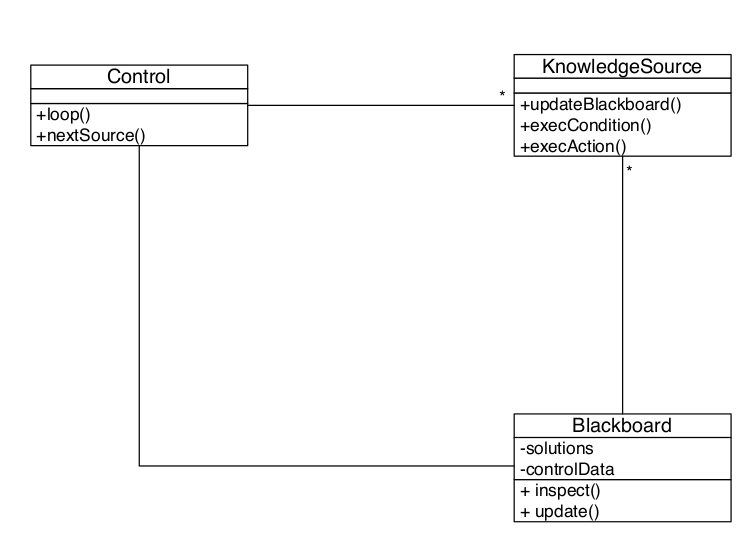
\includegraphics[width=\linewidth]{images/pattern_blackboard.png}
The knowledge sources inspect the current content of the blackboard and create new hypotheses.
Control handles the control flow of the knowledge sources.\\
The blackboard pattern is used when no algorithm for the problem is known.\\
\\
\textbf{6 Steps to Realize a Blackboard Pattern}
\begin{enumerate}
  \item Define the Problem (Identify the application domain, the requirements and the actors)
  \item Define the solution space (top-level and intermediate)
  \item Identify the knowledge sources
  \item Define the blackboard (not every information has to be understandable for every knowledge source)
  \item Define control
  \item Implement the knowledge sources (split into condition part and action part, use computational intelligence or conventional methods)
\end{enumerate}
\newpage

\subsection{Client-Dispatcher-Server Pattern}
The client-dispatcher-server pattern decouples the client from the server.
Usually the client had to know where the server is, now the server is even dynamically interchangeable (server registers to the dispatcher on startup/runtime) what is good for re-configurations and fault tolerance.\\
\begin{minipage}{.5\textwidth}
  Structure:\\
  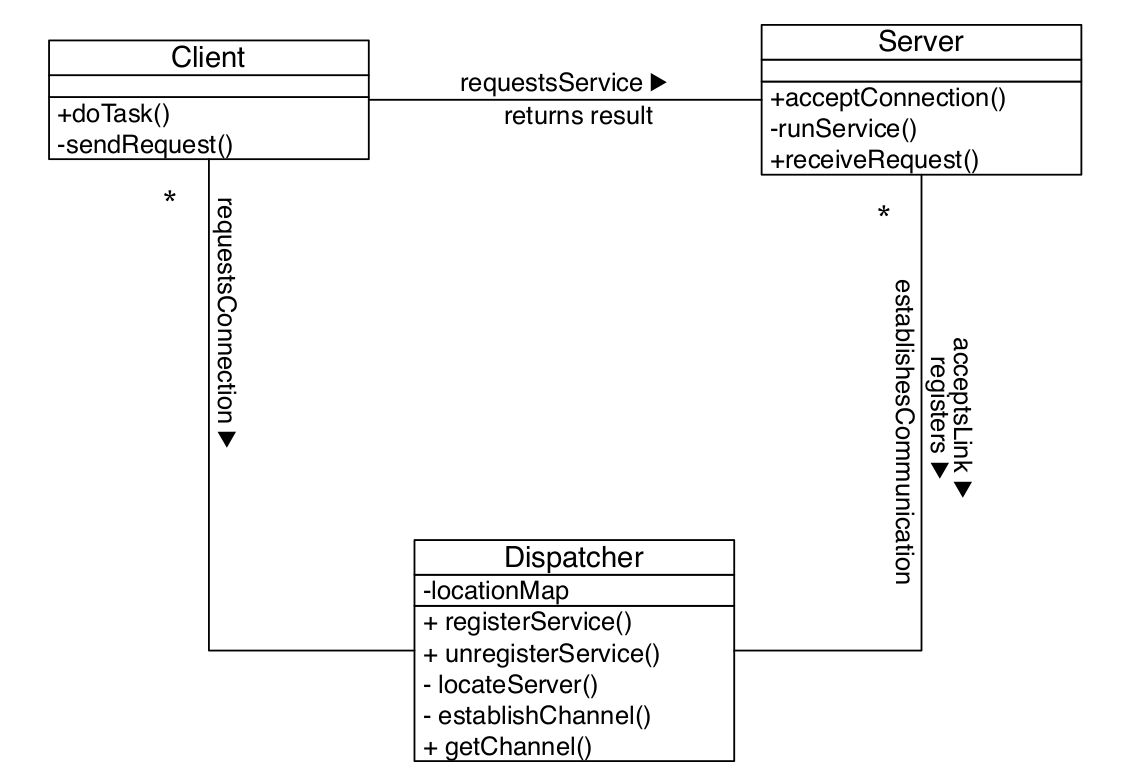
\includegraphics[width=\linewidth]{images/pattern_client_dispatcher_server.png}\\
\end{minipage}
\begin{minipage}{.5\textwidth}
  \vspace{1em}
  Eventflow:\\
  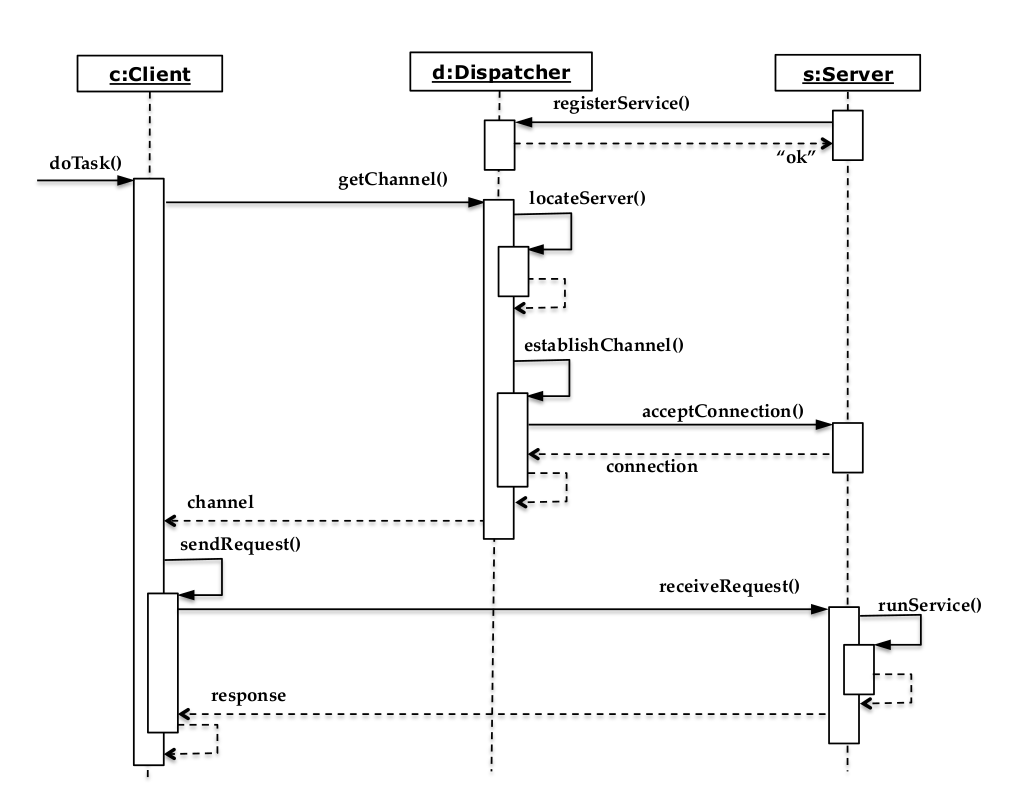
\includegraphics[width=\linewidth]{images/eventflow_client_dispatcher_server.png}
\end{minipage}\\
\\
\textbf{Communication Protocols:}
\begin{description}
  \item[CDprotocol:] Specifies how to ask for servers and handles communication errors.
  \item[DSprotocol:] Specifies how the server registers with the dispatcher and determines the step necessary for a client to establish a connection.
  \item[CSprotocol:] Specifies the communication between client and server.
\end{description}

\textbf{6 Steps to Implement Client-Dispatcher-Server}
\begin{enumerate}
  \item During system design identify the subsystems that act as clients and servers
  \item Decide on the communication mechanism to be used for the protocols (Shared memory, sockets)
  \item Specify the protocols
  \item Decide on a naming scheme for the dispatcher (URLs are ok, IPs not)
  \item Implement the dispatcher
  \begin{enumerate}
    \item Decide how to implement the 3 protocols (sockets, RPM)
    \item Implement requests, responses and errors
    \item Implement a repository that maps server names to addresses
  \end{enumerate}
  \item Implement the client and server (also: when does the server register? Startup or runtime?)
\end{enumerate}
\newpage

\subsection{Broker Pattern}
The broker pattern coordinates the communication between heterogeneous nodes.\\
\\
\textbf{Nonfunctional Requirements:}\\
\vspace{-1.5em}
\begin{description}
  \item[Low Coupling:] Decoupling of service and communication
  \item[Location Transparency:] Services are independent of the server location
  \item[Runtime Extensibility:] Ability to add, remove, exchange components at runtime
  \item[Platform Transparency:] Clients and servers can be written in different languages.
\end{description}
Structure:\\
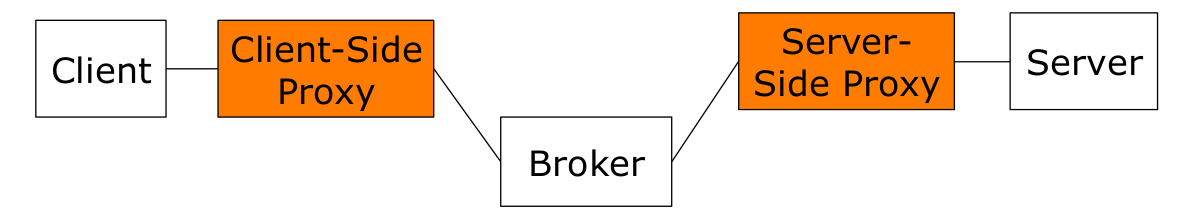
\includegraphics[width=\linewidth]{images/pattern_broker.png}
\textbf{Client-Side Proxy:} Lets the remote object appear as local one, hides the inter-process communication details used for message transfer between client and broker and provides (un-)marshalling/(de-)serialization of parameters and results.\\
\textbf{Server-Side Proxy:} Same as Client-Side proxy only for the server.\\
Eventflow:\\
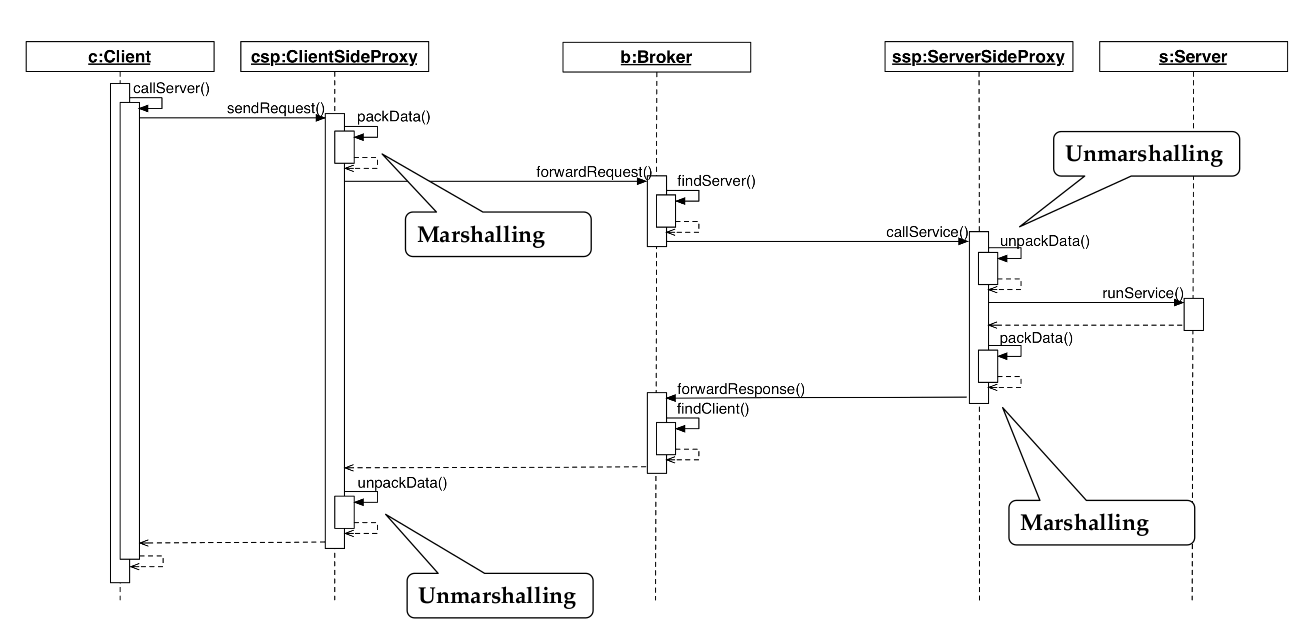
\includegraphics[width=\linewidth]{images/eventflow_broker.png}
\textbf{Steps to Realize a Broker Pattern:}
\begin{enumerate}
  \item Provide the object model and service definitions.
  \item Define the broker service.
  \item Implement the broker component and proxy object at the client and server side.
  \item Implement the client and server.
\end{enumerate}


\newpage

%!tex root = ../report.tex

\section{Antipatterns}
\textbf{Developer antipatterns:}
Focus on the viewpoint of the software developer.\\
Issues: software refactoring, modification of source code to
improve the software structure with respect to long-term
maintainability.\\
\textbf{Architecture antipatterns}
Focus on the viewpoint of the software architect.\\
Issues: partitioning of subsystems and components, platform
independent definition of interfaces, and connectivity of
components.\\
\textbf{Management antipatterns}
Focus on the viewpoint of the software project manager.\\
Issues: software project organization, software project
management, software process model, human communication,
rationale management and resolution of issues.\\

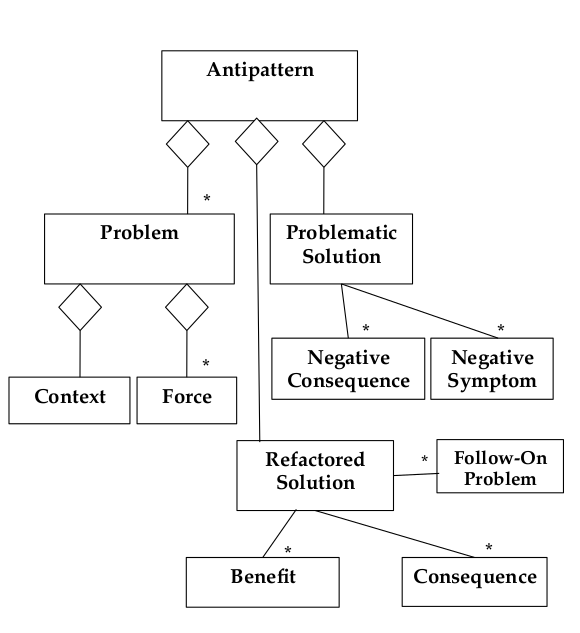
\includegraphics[width=.5\linewidth]{images/antipattern.png}

\textbf{7 Deadly Sins in Software Practice:}
\begin{description}
  \item[Apathy] Not caring about a problem, followed by unwillingness To attempt a solution
  \item[Haste] Solutions based on hasty decisions lead to compromises in software quality
  \item[Narrow-mindedness] The refusal to use solutions that are widely known
  \item[Sloth] Making poor decisions based on "easy" answeres
  \item[Avarice (excessive complexity)] no use of abstractions, excessive modeling of details
  \item[Ignorance] Failure to seek understanding
  \item[Pride] Not invented here: not willing to adopt anything from the outside
\end{description}
\newpage

\subsection{Functional Decomposition Antipattern}
Functional decomposition describes the decomposition of a system in terms of functions instead of use cases and/or objects (object-oriented decomposition) so that functions are hidden somewhere in the system where nobody might expect them.\\
recommended approach: first decompose in use cases, then in objects.
\begin{description}
  \item[General Form] Everything is a function, lots of files named misc, util,aux,...
  \item[Symptoms and Consequences] \hfill
  \begin{itemize}
    \item Maintainer must understand the whole system to make changes
     \item Code is hard to understand
     \item Code is complex, high coupling between code sections in different files
     \item User interface is often awkward and non-intuitive
  \end{itemize}
  \item[Typical Causes] Wrong trained personal (programmers, designers)
\end{description}
\newpage

\subsection{Golden Hammer Antipattern}
Everything is solved with a specific tool.
\begin{description}
  \item[General Form] \hfill
  \begin{itemize}
    \item Developer has high level of competence in a particular solution
    \item Every new development effort is solved with this solution
    \item Developer is unwilling to learn and apply new approach
  \end{itemize}
  \item[Symptoms and Consequences] \hfill
  \begin{itemize}
    \item Identical tools used for a many divers products
    \item System architecture depends on a specific tool chain
  \end{itemize}
  \item[Typical Causes] Large investment in product for specific technologies maybe with exclusive features.
  \item[Known Exceptions] Product is part of a vendor suite that provides for all needs
\end{description}
\newpage

\subsection{Lava Flow}
Also known as dead code.
\begin{description}
  \item[General Form] Lavalike flows of previous development hardened into a basaltlike mass of code, difficult to remove once solidified
  \item[Symptoms and Consequences] \hfill
  \begin{itemize}
    \item Unused or commented-out code
    \item Undocumented complex, important-looking code
    \item Functions or classes that do not relate to the system architecture
    \item evolving architecture
  \end{itemize}
  \item[Typical Causes] \hfill
  \begin{itemize}
    \item Research and development code placed into production
    \item Implementation of several trial approaches
    \item High programmer turnover rate
    \item Fear of breaking something and not knowing how to fix it
    \item Unclear, repeatedly changing project goals
    \item Architectural scars
  \end{itemize}
  \item[Exceptions] Throwaway code
\end{description}
\newpage

\subsection{Blob Antipattern}
Also known as god class
\begin{description}
  \item[General Form] Majority of responsibilities are in one complex controller associated with simple data classes
  \item[Symptoms and Consequences] \hfill
  \begin{itemize}
    \item Huge class with many unrelated attributes and operations encapsulated
    \item The blob is usually to complex to reuse and test
  \end{itemize}
  \item[Typical Causes] \hfill
  \begin{itemize}
    \item Lack of architecture
    \item Too limited intervention in iterative projects
  \end{itemize}
  \item[Known Exceptions] Wrapping of legacy systems
\end{description}
\newpage

%!TEX root = ../report.tex

\section{Comparisons}

\subsection{Adapter vs. Bridge}
Both hide the detail of the underlying implementation, but:
\begin{itemize}
   \item the adapter (inheritance followed by delegation) is designed to handle incompatibilities
   \item the bridge (delegation followed by inheritance) is intended to differentiate between abstraction and implementation up-front
 \end{itemize}

 \subsection{Bridge vs. Strategy}
 The bridge is used for structural decisions on system startup whereas the strategy handles behavioral decisions on runtime based on changing criteria.

\subsection{Strategy vs. State}
The strategy pattern handles different algorithms at runtime whereas the state pattern handles different states of an object in the architecture.

\newpage

%!TEX root = ../report.tex

\section{Terminology}
\begin{description}
  \item[Coupling] measures the dependencies between subsystems

  \item[Cohesion] Measures the dependencies among classes within a subsystem

  \item[Design Pattern] describes associations and collaborations of a set of classes.

  \item[Architectural Style] is a pattern for a subsystem decomposition, i.e. describes relationships and collaborations of different subsystems.

  \item[Software Architecture] is an instance of an architectural style.

  \item[User Model] is imagined by the user in their mind.
  It helps the user to know and understand the underlaying application domain model.

  \item[Natural Mapping (UI)] is a mapping between UI controls of a system and objects in the real world such that the mapping does not tax the user's memory when performing a task that involves the manipulation of these controls.

  \item[Components/Subsystems] Computational units with a specified interface

  \item[Connectors/Communication] Interactions between the components/subsystems
\end{description}


% Needs to be enabled when there are any references.
% \clearpage
% \addcontentsline{toc}{section}{\refname}
% \printbibliography

\end{document}
